\chapter{जनन का हॉर्मोनी नियंत्रण}\label{ch:g11:hormones-and-reproduction}

कोई स्त्री एक चार्ट रखती है: हर सुबह अपना ताप, जिसमें हर महीने के बीचोबीच
एक छोटी-सी चढ़ाई आती है; और हर अट्ठाईस दिन के आसपास एक रक्तस्राव। यदि कोई
प्रयोगशाला उसके रक्त में चार \omterm{def:g11:hormones-and-reproduction:hormone}{हॉर्मोन} हर दिन नापे तो वह चार ऐसे वक्र खींचती
जो एक तय क्रम में, महीने-दर-महीने चढ़ते और गिरते हैं, और जिनकी हर चोटी
अगली को पैदा करती है। किसी पुरुष का प्रयोगशाला चार्ट वही \omterm{def:g11:hormones-and-reproduction:hormone}{हॉर्मोन} दिन-दर-दिन
लगभग स्थिर स्तरों पर दिखाता। अंग अलग हैं; पर नियंत्रण की व्यवस्था ---
मस्तिष्क का एक केंद्र, उसके नीचे एक ग्रंथि, जननग्रंथि, और दोनों दिशाओं में
रक्त के ढोए संदेश --- वही है। यह अध्याय वे चार्ट पढ़ता है, और दिखाता है कि
उन्हें समझ लेने से किसी गर्भ को रोकना, या पाना, कैसे संभव हो गया।

\section{हॉर्मोन और उनके फंदे}

\begin{definition}[हॉर्मोन, प्रतिपुष्टि]\label{def:g11:hormones-and-reproduction:hormone}
\emph{हॉर्मोन}\index{हॉर्मोन} वह अणु है जो कोई ग्रंथि रक्त में स्रावित
करती है और जो दूर से, उन \omterm{def:g10:cells-common-unit:cell}{कोशिकाओं} पर काम करता है जो उसका कोई
\emph{ग्राही} ढोती हों। किसी हॉर्मोनी व्यवस्था को
\emph{प्रतिपुष्टि}\index{प्रतिपुष्टि} नियंत्रित करती है: किसी शृंखला के
अंत में बना हॉर्मोन पलटकर उसके आरंभ की ग्रंथियों पर काम करता है।
\emph{ऋणात्मक प्रतिपुष्टि} --- यानी उत्पाद आदेश घटा देता है --- किसी स्तर
को स्थिर रखती है; और \emph{धनात्मक प्रतिपुष्टि} --- यानी उत्पाद आदेश बढ़ा
देता है --- कोई उछाल पैदा करती है।
\end{definition}

\begin{proposition}[साझा शृंखला]\label{prop:g11:hormones-and-reproduction:chain}
दोनों लिंगों में जननग्रंथियों को वही तीन-मंज़िला शृंखला नियंत्रित करती है।
मस्तिष्क का एक केंद्र, यानी \emph{अधश्चेतक}, स्पंदों में एक विमोचक
\omterm{def:g11:hormones-and-reproduction:hormone}{हॉर्मोन}, GnRH, उन छोटी वाहिकाओं में स्रावित करता है जो उसके ठीक नीचे की
\emph{पीयूष ग्रंथि} तक जाती हैं; पीयूष ग्रंथि इसके जवाब में दो \omterm{def:g11:hormones-and-reproduction:hormone}{हॉर्मोन},
\emph{LH} और \emph{FSH}, आम रक्त में स्रावित करती है; और ये जननग्रंथियों
पर काम करते हैं, जो युग्मक भी बनाती हैं और लैंगिक \omterm{def:g11:hormones-and-reproduction:hormone}{हॉर्मोन} भी --- वृषण में
\omterm{prop:g11:becoming-male-female:hormones}{टेस्टोस्टेरोन}, और अंडाशय में एस्ट्रोजन तथा प्रोजेस्टेरोन। ये लैंगिक
\omterm{def:g11:hormones-and-reproduction:hormone}{हॉर्मोन} शरीर पर काम करते हैं, और पलटकर अधश्चेतक तथा पीयूष ग्रंथि पर भी।
\end{proposition}
\admitted

\section{नर: एक स्थिर स्तर}

\begin{proposition}[वृषण का नियंत्रण]\label{prop:g11:hormones-and-reproduction:male}
वृषण के दो खाने हैं। \emph{शुक्रजनक नलिकाएँ}, जिन्हें FSH और
\omterm{prop:g11:becoming-male-female:hormones}{टेस्टोस्टेरोन} उकसाते हैं, \omterm{prop:g11:becoming-male-female:puberty}{यौवनारंभ} से लगातार शुक्राणु बनाती हैं, यानी
रोज़ाना क़रीब दस करोड़। और नलिकाओं के बीच की \omterm{def:g10:cells-common-unit:cell}{कोशिकाएँ}, जिन्हें LH उकसाता है,
\emph{\omterm{prop:g11:becoming-male-female:hormones}{टेस्टोस्टेरोन}} स्रावित करती हैं, जो जनन तंत्र, गौण लक्षणों और
शुक्राणु-निर्माण को बनाए रखता है। \omterm{prop:g11:becoming-male-female:hormones}{टेस्टोस्टेरोन} अधश्चेतक और पीयूष ग्रंथि को
दबाता है: वह चढ़े तो GnRH, LH और FSH गिरते हैं और वृषण कम स्रावित करता है;
और वह गिरे तो वे चढ़ जाते हैं। यही ऋणात्मक \omterm{def:g11:hormones-and-reproduction:hormone}{प्रतिपुष्टि} उस स्तर को,
रोज़मर्रा के छोटे उतार-चढ़ावों के भीतर, \omterm{prop:g11:becoming-male-female:puberty}{यौवनारंभ} से बुढ़ापे तक लगभग स्थिर
रखती है।
\end{proposition}
\begin{proof}[साक्ष्य]
किसी जानवर की जननग्रंथियाँ हटा देने से उसका LH कुछ ही दिनों में कई गुना चढ़
जाता है; और \omterm{prop:g11:becoming-male-female:hormones}{टेस्टोस्टेरोन} का इंजेक्शन उसे दोबारा नीचे ले आता है। अधश्चेतक
की कोई क्षति LH, FSH और \omterm{prop:g11:becoming-male-female:hormones}{टेस्टोस्टेरोन}, तीनों मिटा देती है; और स्पंदों में
GnRH इंजेक्ट करने से तीनों लौट आते हैं, जबकि GnRH के लगातार बहाव से नहीं
--- यानी स्पंदन मायने रखता है। जिन पुरुषों को किसी और वजह से
\omterm{prop:g11:becoming-male-female:hormones}{टेस्टोस्टेरोन} दिया जाता है उनका शुक्राणु-निर्माण गिरता देखा जाता है: बाहर
से आया वह \omterm{def:g11:hormones-and-reproduction:hormone}{हॉर्मोन} उनकी अपनी पीयूष ग्रंथि बंद कर देता है।
\end{proof}

\begin{omfigure}
\begin{tikzpicture}[font=\small, >=Stealth,
  b/.style={draw, rounded corners, align=center, text width=2.8cm, minimum height=1.0cm}]
  \node[b, fill=omDef!12] (h) at (0,3.2) {अधश्चेतक};
  \node[b, fill=omDef!12] (p) at (0,1.6) {पीयूष ग्रंथि};
  \node[b, fill=omProp!15] (t) at (0,0) {वृषण};
  \node[b, fill=omMeth!15, text width=3.6cm] (body) at (6.0,0) {शुक्राणु-निर्माण;\\ तंत्र, गौण\\ लक्षण};
  \draw[->, thick] (h) -- node[right] {GnRH (स्पंद)} (p);
  \draw[->, thick] (p) -- node[right] {LH, FSH} (t);
  \draw[->, thick] (t) -- node[above] {टेस्टोस्टेरोन} (body);
  \draw[->, thick, omThm, rounded corners=4pt] (t.west) -- (-2.3,0) -- (-2.3,3.2) -- (h.west);
  \node[omThm, anchor=east, align=right] at (-2.45,1.6) {टेस्टोस्टेरोन\\ दबाता है};
  \draw[->, thick, omThm] (-2.3,1.6) -- (p.west);
  \node[omThm, font=\scriptsize] at (-0.7,0.35) {$-$};
\end{tikzpicture}

{\small वृषण का नियंत्रण। अधश्चेतक पीयूष ग्रंथि को चलाता है, पीयूष ग्रंथि
वृषण को, और वृषण का \omterm{prop:g11:becoming-male-female:hormones}{टेस्टोस्टेरोन} दोनों को दबाता है: यानी ऋणात्मक
\omterm{def:g11:hormones-and-reproduction:hormone}{प्रतिपुष्टि} का एक फंदा, जो \omterm{prop:g11:becoming-male-female:hormones}{टेस्टोस्टेरोन} को लगभग स्थिर रखता है।}
\end{omfigure}

\section{मादा: चक्र}

\begin{proposition}[अंडाशय का चक्र]\label{prop:g11:hormones-and-reproduction:ovary}
\omterm{prop:g11:becoming-male-female:puberty}{यौवनारंभ} से रजोनिवृत्ति तक अंडाशय लगभग 28 दिन का एक चक्र चलाता है।
\begin{itemize}
  \item \emph{पुटकीय प्रावस्था} (दिन 1--13): FSH के नीचे कोई पुटक ---
        यानी अपनी पोषक \omterm{def:g10:cells-common-unit:cell}{कोशिकाओं} से घिरा एक अंडाणु --- बढ़ता है और चढ़ती
        मात्रा में \emph{एस्ट्रोजन} स्रावित करता है।
  \item \emph{अंडोत्सर्ग} (दिन 14): LH का एक उछाल परिपक्व पुटक को फोड़
        देता है, जो अपना अंडाणु अंडवाहिनी में छोड़ देता है।
  \item \emph{पीत प्रावस्था} (दिन 15--28): ख़ाली हुआ पुटक \emph{पीत पिंड}
        बन जाता है, जो \emph{प्रोजेस्टेरोन} और एस्ट्रोजन स्रावित करता है;
        और यदि कोई गर्भ शुरू न हो तो वह क़रीब बारह दिन बाद क्षीण हो जाता
        है, दोनों \omterm{def:g11:hormones-and-reproduction:hormone}{हॉर्मोन} गिर जाते हैं, और एक नया चक्र शुरू हो जाता है।
\end{itemize}
\end{proposition}
\admitted

\begin{omfigure}
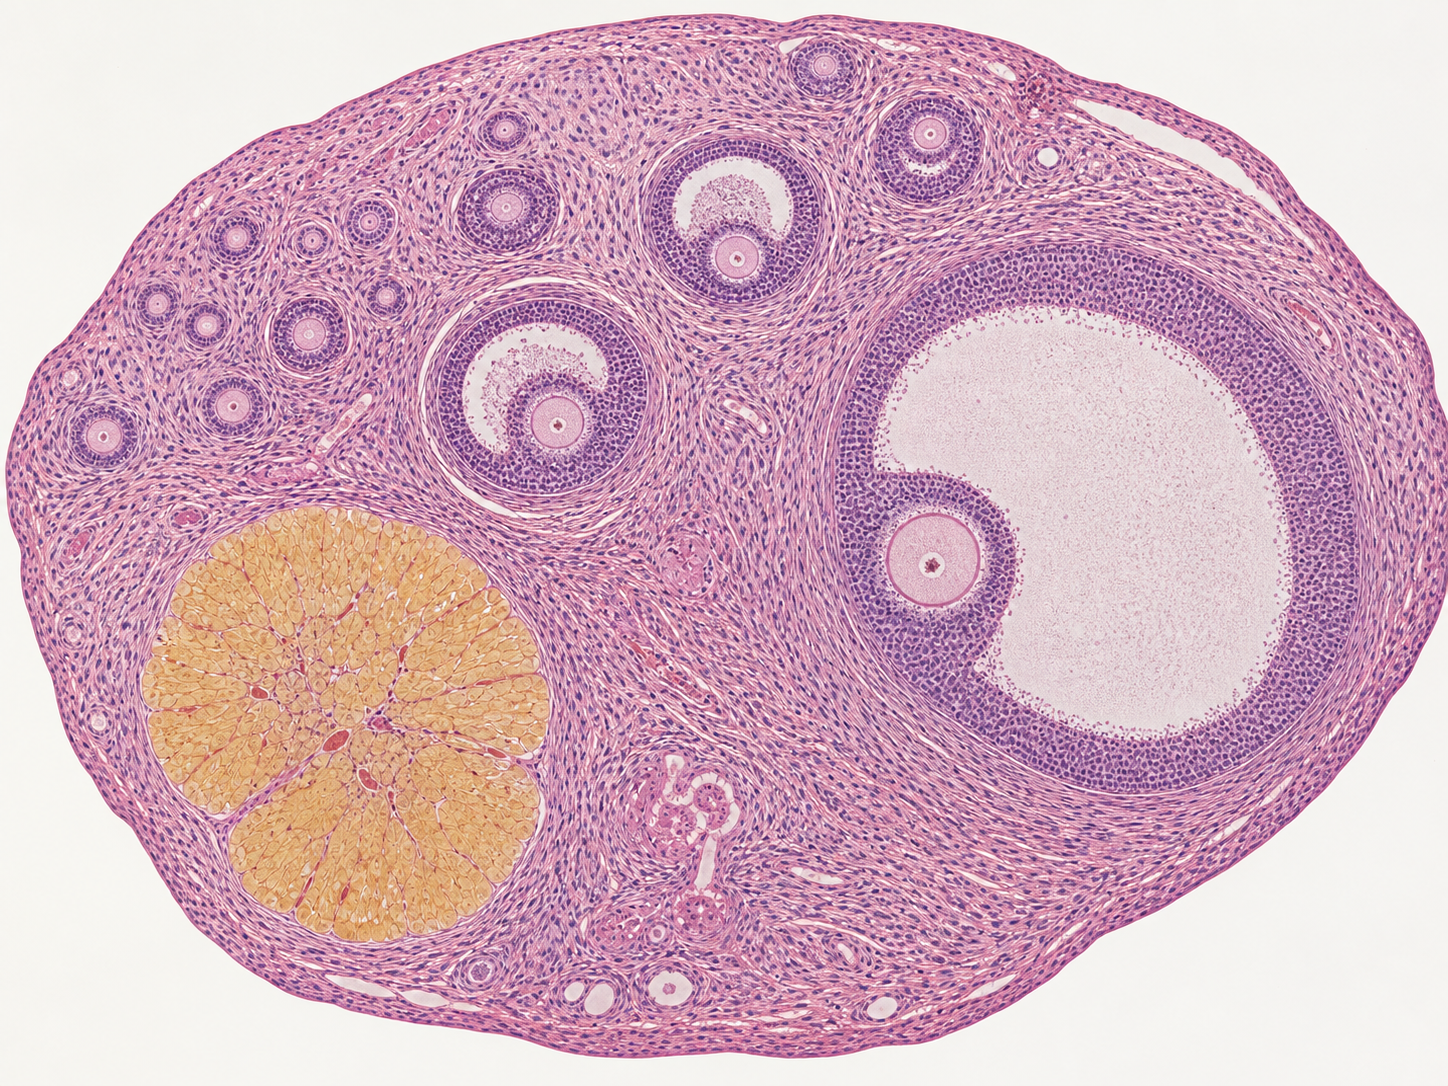
\includegraphics[width=0.56\linewidth]{images/book2/ai/g11-ovary-section.png}

{\small अंडाशय की एक काट: वृद्धि की एक के बाद एक अवस्थाओं में पुटक, और उनमें
सबसे बड़ा अपनी तरल-भरी गुहा तथा भीतर के अंडाणु के साथ, और एक पीत पिंड ---
यानी उस पुटक का अवशेष जो अंडोत्सर्ग कर चुका है।}
\end{omfigure}

\begin{proposition}[गर्भाशय का चक्र और प्रतिपुष्टियाँ]\label{prop:g11:hormones-and-reproduction:uterus}
गर्भाशय की परत अंडाशय के \omterm{def:g11:hormones-and-reproduction:hormone}{हॉर्मोनों} के पीछे चलती है: पुटकीय प्रावस्था के
दौरान एस्ट्रोजन उसे मोटा करते हैं; पीत प्रावस्था के दौरान प्रोजेस्टेरोन उसे
स्रावी और किसी भ्रूण को लेने लायक़ बना देता है; और चक्र के अंत में दोनों का
गिरना उसे टूटकर बहने पर मजबूर कर देता है --- यानी \emph{मासिक धर्म}, जो
अगले चक्र के दिन 1 से 5 तक चलता है। चक्र के दौरान \omterm{def:g11:hormones-and-reproduction:hormone}{प्रतिपुष्टियाँ} अपना चिह्न
बदल लेती हैं: कम और मध्यम स्तरों पर एस्ट्रोजन तथा प्रोजेस्टेरोन अधश्चेतक और
पीयूष ग्रंथि को दबाते हैं (ऋणात्मक \omterm{def:g11:hormones-and-reproduction:hormone}{प्रतिपुष्टि}); पर परिपक्व पुटक का ऊँचा
एस्ट्रोजन, दो दिन तक टिका रहे तो, उन्हें \emph{उकसाता} है (धनात्मक
\omterm{def:g11:hormones-and-reproduction:hormone}{प्रतिपुष्टि}), और यही LH का वह उछाल पैदा करता है जो अंडोत्सर्ग करा देता है।
अंडोत्सर्ग के बाद पीत पिंड का प्रोजेस्टेरोन ऋणात्मक \omterm{def:g11:hormones-and-reproduction:hormone}{प्रतिपुष्टि} लौटा देता
है, और कोई दूसरा उछाल नहीं आता।
\end{proposition}
\begin{proof}[साक्ष्य]
रोज़ाना की रक्त-मापें अगले चित्र के वक्र देती हैं: LH का उछाल एस्ट्रोजन की
चोटी के एक दिन बाद आता है और अंडोत्सर्ग से एक दिन पहले; और प्रोजेस्टेरोन
केवल अंडोत्सर्ग के बाद उभरता है। अंडाशय हटा देने से LH और FSH चढ़ जाते हैं;
एस्ट्रोजन की छोटी ख़ुराकें उन्हें गिरा देती हैं; और चक्र के बीच में दी गई
कोई बड़ी, टिकी हुई ख़ुराक LH का उछाल भड़का देती है --- यानी ख़ुराक के साथ
\omterm{def:g11:hormones-and-reproduction:hormone}{प्रतिपुष्टि} का चिह्न पलट जाता है। जिस स्त्री की पीयूष ग्रंथि एस्ट्रोजन की
चढ़ाई का जवाब न दे सके उसमें कोई उछाल नहीं आता और अंडोत्सर्ग नहीं होता,
हालाँकि उसके पुटक बढ़ते हैं।
\end{proof}

\begin{omfigure}
\begin{tikzpicture}
\begin{axis}[
  width=0.92\linewidth, height=6.4cm,
  axis x line=bottom, axis y line=left,
  xmin=0, xmax=28, ymin=0, ymax=122,
  xlabel={चक्र का दिन}, ylabel={हॉर्मोन (अपने अधिकतम का \%)},
  xlabel style={font=\small, at={(axis description cs:0.5,-0.1)}, anchor=north},
  ylabel style={font=\small},
  tick label style={font=\small}, xtick={0,7,14,21,28}, ytick={0,50,100},
  legend style={at={(0.5,-0.22)}, anchor=north, legend columns=4, font=\small, draw=none},
  clip=false,
]
\addplot[thick, omMeth, smooth] coordinates {(0,10) (4,15) (8,30) (11,70) (12,100) (13,80) (14,45) (16,35) (19,55) (22,60) (25,40) (28,10)};
\addplot[thick, omProp, smooth] coordinates {(0,3) (12,3) (14,5) (16,30) (19,70) (21,100) (23,90) (25,55) (27,15) (28,5)};
\addplot[thick, omThm] coordinates {(0,15) (11,18) (12,35) (13,100) (14,60) (15,15) (28,12)};
\addplot[thick, omDef, dashed] coordinates {(0,45) (4,40) (9,30) (12,35) (13,70) (14,45) (15,20) (28,25)};
\draw[dashed, gray] (axis cs:14,0) -- (axis cs:14,113);
\node[font=\small, anchor=south] at (axis cs:14,113) {अंडोत्सर्ग};
\draw[<->, gray] (axis cs:0.3,104) -- (axis cs:13.7,104);
\node[font=\scriptsize, anchor=south] at (axis cs:7,105) {पुटकीय प्रावस्था};
\draw[<->, gray] (axis cs:14.3,104) -- (axis cs:27.7,104);
\node[font=\scriptsize, anchor=south] at (axis cs:21,105) {पीत प्रावस्था};
\legend{एस्ट्रोजन, प्रोजेस्टेरोन, LH, FSH}
\end{axis}
\end{tikzpicture}

{\small एक चक्र के \omterm{def:g11:hormones-and-reproduction:hormone}{हॉर्मोन}। एस्ट्रोजन बढ़ते पुटक के साथ चढ़ते हैं और दिन 12
पर चोटी छूते हैं; LH का उछाल दिन 13 पर आता है और अंडोत्सर्ग दिन 14 पर; और
पीत पिंड का प्रोजेस्टेरोन दूसरे आधे पर छाया रहता है तथा अंत में गिरकर मासिक
धर्म ले आता है।}
\end{omfigure}

\begin{omfigure}
\begin{tikzpicture}[font=\small, >=Stealth,
  b/.style={draw, rounded corners, align=center, text width=2.8cm, minimum height=1.0cm}]
  \node[b, fill=omDef!12] (h) at (0,3.2) {अधश्चेतक};
  \node[b, fill=omDef!12] (p) at (0,1.6) {पीयूष ग्रंथि};
  \node[b, fill=omProp!15] (o) at (0,0) {अंडाशय};
  \node[b, fill=omMeth!15, text width=3.4cm] (u) at (6.4,0) {गर्भाशय की परत:\\ मोटी होती है, फिर\\ भ्रूण के लिए तैयार};
  \draw[->, thick] (h) -- node[right] {GnRH} (p);
  \draw[->, thick] (p) -- node[right] {FSH, LH} (o);
  \draw[->, thick] (o) -- node[above, align=center] {एस्ट्रोजन,\\ प्रोजेस्टेरोन} (u);
  \draw[->, thick, omThm, rounded corners=4pt] (o.west) -- (-2.3,0) -- (-2.3,3.2) -- (h.west);
  \node[omThm, anchor=east, align=right, text width=2.6cm] at (-2.45,0.9) {कम या मध्यम स्तर दबाते हैं $(-)$};
  \draw[->, thick, omThm] (-2.3,1.6) -- (p.west);
  \draw[->, thick, omMeth!70!black] (o.north west) .. controls (-2.0,0.9) and (-2.0,2.3) .. (h.south west);
  \node[omMeth!70!black, font=\scriptsize, anchor=east, align=right, text width=2.4cm] at (-2.45,2.7) {दो दिन तक ऊँचा एस्ट्रोजन उकसाता है $(+)$: LH उछाल};
\end{tikzpicture}

{\small अंडाशय का नियंत्रण। नर वाली ही शृंखला, पर ऐसी \omterm{def:g11:hormones-and-reproduction:hormone}{प्रतिपुष्टि} के साथ जो
अपना चिह्न बदल लेती है: महीने भर ऋणात्मक, और एस्ट्रोजन की चोटी वाले उन दो
दिनों के लिए धनात्मक, जो LH का उछाल तथा अंडोत्सर्ग करा देते हैं।}
\end{omfigure}

\begin{method}[चक्र का चार्ट पढ़ना]\label{met:g11:hormones-and-reproduction:read}
\begin{enumerate}
  \item LH की चोटी ढूँढ़िए: अंडोत्सर्ग उसके अगले दिन है; उससे पहले सब कुछ
        पुटकीय प्रावस्था है और उसके बाद सब कुछ पीत प्रावस्था।
  \item क्रम जाँचिए: एस्ट्रोजन की चोटी, फिर LH का उछाल, फिर अंडोत्सर्ग,
        फिर प्रोजेस्टेरोन। क्रम से बाहर कोई वक्र किसी गड़बड़ी का निशान है।
  \item गिनिए: पीत प्रावस्था हर स्त्री में 14 दिन के क़रीब होती है; और
        चक्र की लंबाई पुटकीय प्रावस्था से बदलती है। इसलिए अंडोत्सर्ग अगले
        मासिक धर्म से 14 दिन पहले होता है, पिछले के 14 दिन बाद नहीं।
  \item किसी दवा या क्षति की व्याख्या यह पूछकर कीजिए कि वह कौन-सा \omterm{def:g11:hormones-and-reproduction:hormone}{हॉर्मोन}
        जोड़ती या हटाती है, और फिर \omterm{def:g11:hormones-and-reproduction:hormone}{प्रतिपुष्टि} बाक़ियों का क्या करती है।
\end{enumerate}
\end{method}

\section{चुनना: गर्भनिरोध}

\begin{proposition}[हॉर्मोनी गर्भनिरोध]\label{prop:g11:hormones-and-reproduction:contraception}
संयुक्त गोली हर दिन किसी एस्ट्रोजन और प्रोजेस्टेरोन जैसे किसी अणु की छोटी
ख़ुराकें देती है। उन स्तरों पर \omterm{def:g11:hormones-and-reproduction:hormone}{प्रतिपुष्टि} पूरे समय ऋणात्मक रहती है: FSH
नीचा बना रहता है, कोई पुटक परिपक्व नहीं होता, एस्ट्रोजन की कोई चोटी नहीं
आती, न LH का उछाल, न अंडोत्सर्ग। पतली रखी गई गर्भाशय की परत और गाढ़ा रखा
गया ग्रीवा का श्लेष्मा दो और अवरोध जोड़ देते हैं। हफ़्ते भर गोलियाँ रोक
देने से वे \omterm{def:g11:hormones-and-reproduction:hormone}{हॉर्मोन} गिर जाते हैं और वह परत बह जाती है। दूसरे तरीक़े कहीं और
काम करते हैं: गर्भाशय में रखा ताँबे का उपकरण निषेचन और रोपण रोक देता है;
संभोग के कुछ ही दिनों के भीतर ली गई आपात गोली अंडोत्सर्ग टाल देती है; और
कंडोम युग्मकों को मिलने से रोक देते हैं --- तथा वही अकेला तरीक़ा हैं जो
यौन-संचरित संक्रमण भी रोकता है।
\end{proposition}
\admitted

\begin{example}[गोली का असर पढ़ना]\label{ex:g11:hormones-and-reproduction:pill}
गोली लेती किसी स्त्री के चार्ट पर चारों वक्र सपाट रहते हैं: एस्ट्रोजन और
प्रोजेस्टेरोन उस नीचे, ठहरे हुए स्तर पर जो गोलियाँ देती हैं, तथा LH और FSH
अपने चक्रीय न्यूनतम से भी नीचे, और कहीं कोई चोटी नहीं। पैकेट के शुरू में
कुछ दिन गोलियाँ चूक जाएँ तो FSH छूट निकलता है: कोई पुटक शुरू हो सकता है,
और उसके बाद बाक़ी सब भी। गोली इसलिए चलती है कि \omterm{def:g11:hormones-and-reproduction:hormone}{प्रतिपुष्टि} चलती है, और भूली
हुई गोली उस \omterm{def:g11:hormones-and-reproduction:hormone}{प्रतिपुष्टि} में एक छेद है।
\end{example}

\section{पाना: सहायता-प्राप्त जनन}

\begin{proposition}[जब गर्भ नहीं ठहरता]\label{prop:g11:hormones-and-reproduction:art}
सात में लगभग एक दंपती साल भर की कोशिश के बाद सलाह लेता है। कारण दोनों की
ओर से आते हैं: अंडोत्सर्ग का न होना या अनियमित होना, बंद अंडवाहिनियाँ, बहुत
कम या गतिहीन शुक्राणु, और एक-तिहाई मामलों में कोई पहचाना हुआ कारण ही नहीं।
इलाज जीवविज्ञान के पीछे चलते हैं:
\begin{itemize}
  \item \emph{अंडोत्सर्ग को उकसाना}: FSH के इंजेक्शन, या ऐसी दवा जो
        एस्ट्रोजन की ऋणात्मक \omterm{def:g11:hormones-and-reproduction:hormone}{प्रतिपुष्टि} रोक दे, पुटकों को परिपक्व कर देते
        हैं; और फिर LH जैसा कोई इंजेक्शन चुने हुए समय पर अंडोत्सर्ग करा
        देता है;
  \item \emph{वीर्यसेचन}: अंडोत्सर्ग के समय तैयार किया गया वीर्य गर्भाशय
        में रख दिया जाता है;
  \item \emph{पात्र-निषेचन}: उकसावे के बाद अंडाणु सुई से अंडाशय से इकट्ठे
        किए जाते हैं, किसी तश्तरी में निषेचित किए जाते हैं --- ज़रूरत हो
        तो हर अंडाणु में एक शुक्राणु इंजेक्ट करके --- और तीन से पाँच दिन
        बाद एक या दो भ्रूण गर्भाशय में रख दिए जाते हैं। तीन या चार में
        लगभग एक कोशिश किसी जन्म तक पहुँचती है; और बाक़ी जमे हुए भ्रूणों
        के साथ दोहराई जा सकती हैं।
\end{itemize}
प्राकृतिक शृंखला का जो भी क़दम चूकता है उसकी जगह उससे मेल खाता हस्तक्षेप ले
लेता है।
\end{proposition}
\admitted

\begin{example}[एक कोशिश के अंक]\label{ex:g11:hormones-and-reproduction:ivf}
उकसावे से 10 अंडाणु मिलते हैं; 8 परिपक्व होते हैं; 5 निषेचित होते हैं; 3
पाँच दिन वाली अवस्था तक पहुँचते हैं; 1 स्थानांतरित किया जाता है और 2 जमा
दिए जाते हैं। वह स्थानांतरण लगभग एक-तिहाई मामलों में सफल होता है; और दोनों
जमे हुए भ्रूणों के साथ उस एक ही संग्रह से जन्म की संभावना बढ़कर क़रीब 60\%
हो जाती है। इस तकनीक ने 1978 से अब तक कई लाख बच्चे दिए हैं; और उसने ऐसे
सवाल भी खड़े किए हैं --- इस्तेमाल न हुए भ्रूणों के बारे में, माता-पिता की
उम्र के बारे में, और क्या-क्या चुना जा सकता है इसके बारे में --- जिनका
जवाब जीवविज्ञान नहीं देता।
\end{example}

\begin{remark}[दो व्यवस्थाएँ जो मिलती हैं]\label{rem:g11:hormones-and-reproduction:brain}
इस अध्याय के \omterm{def:g11:hormones-and-reproduction:hormone}{हॉर्मोन} जननग्रंथियों और शरीर को नियंत्रित करते हैं; पर वे
मनुष्यों में यौन व्यवहार को उस तरह नियंत्रित नहीं करते जैसे बहुत-से जानवरों
में करते हैं, जिनमें संगम अंडाशय के चक्र से बँधा है। मनुष्य की यौन क्रिया
बड़े हिस्से में उस चक्र से स्वतंत्र है और मस्तिष्क की इच्छा, सुख तथा लगाव
की व्यवस्थाओं पर निर्भर है --- यानी इनाम के उन परिपथों पर जो दूसरी
प्रेरणाओं के साथ साझा हैं --- तथा उस व्यक्ति के इतिहास, संस्कृति और चुनावों
पर। जनन और यौनिकता एक-दूसरे को छूते हैं; पर वे एक ही चीज़ नहीं हैं, और
\omterm{def:g11:hormones-and-reproduction:hormone}{हॉर्मोन} केवल पहली को चलाते हैं।
\end{remark}

\section{अभ्यास}

\begin{exercise}[$\star$]\label{exo:g11:hormones-and-reproduction:1}
\omterm{def:g11:hormones-and-reproduction:hormone}{हॉर्मोन} और \omterm{def:g11:hormones-and-reproduction:hormone}{प्रतिपुष्टि} की परिभाषा दीजिए, और ऋणात्मक तथा धनात्मक
\omterm{def:g11:hormones-and-reproduction:hormone}{प्रतिपुष्टि} में अंतर बताइए।
\end{exercise}

\begin{exercise}[$\star$]\label{exo:g11:hormones-and-reproduction:2}
जननग्रंथियों को नियंत्रित करती शृंखला की तीनों मंज़िलों के नाम लिखिए और हर
एक जो \omterm{def:g11:hormones-and-reproduction:hormone}{हॉर्मोन} स्रावित करती है वह भी।
\end{exercise}

\begin{exercise}[$\star$]\label{exo:g11:hormones-and-reproduction:3}
वृषण के दोनों खाने कौन-से हैं और हर एक क्या बनाता है?
\end{exercise}

\begin{exercise}[$\star$]\label{exo:g11:hormones-and-reproduction:4}
अंडाशय के चक्र की प्रावस्थाएँ उनके \omterm{def:g11:hormones-and-reproduction:hormone}{हॉर्मोनों} समेत गिनाइए।
\end{exercise}

\begin{exercise}[$\star$]\label{exo:g11:hormones-and-reproduction:5}
मासिक धर्म किससे होता है?
\end{exercise}

\begin{exercise}[$\star\star$]\label{exo:g11:hormones-and-reproduction:6}
चक्र वाले चित्र से एस्ट्रोजन की चोटी, LH की चोटी, अंडोत्सर्ग और
प्रोजेस्टेरोन की चोटी के दिन बताइए।
\end{exercise}

\begin{exercise}[$\star\star$]\label{exo:g11:hormones-and-reproduction:7}
समझाइए कि जननग्रंथियाँ हटाने से LH क्यों चढ़ जाता है, और \omterm{prop:g11:becoming-male-female:hormones}{टेस्टोस्टेरोन} का
इंजेक्शन उसे दोबारा क्यों गिरा देता है।
\end{exercise}

\begin{exercise}[$\star\star$]\label{exo:g11:hormones-and-reproduction:8}
समझाइए कि दिन 12 की एस्ट्रोजन चोटी LH का उछाल क्यों पैदा करती है, जबकि
दिन 20 का एस्ट्रोजन नहीं करता।
\end{exercise}

\begin{exercise}[$\star\star$]\label{exo:g11:hormones-and-reproduction:9}
किसी स्त्री के चक्र 35 दिन के हैं। वह किस दिन अंडोत्सर्ग करती है? कारण
बताइए।
\end{exercise}

\begin{exercise}[$\star\star$]\label{exo:g11:hormones-and-reproduction:10}
\omterm{def:g11:hormones-and-reproduction:hormone}{प्रतिपुष्टि} के चिह्न की मदद से समझाइए कि संयुक्त गोली अंडोत्सर्ग कैसे रोक
देती है।
\end{exercise}

\begin{exercise}[$\star\star$]\label{exo:g11:hormones-and-reproduction:11}
शरीर-सौष्ठव के लिए \omterm{prop:g11:becoming-male-female:hormones}{टेस्टोस्टेरोन} लेते किसी पुरुष के वृषण सिकुड़ते और
शुक्राणुओं की गिनती गिरती दिखती है। समझाइए।
\end{exercise}

\begin{exercise}[$\star\star\star$]\label{exo:g11:hormones-and-reproduction:12}
कोई दवा अधश्चेतक के एस्ट्रोजन-ग्राही रोक देती है। FSH पर, पुटकों की वृद्धि
पर और अंडोत्सर्ग पर उसके असर का अनुमान लगाइए, और बताइए कि वह कुछ बंध्यताओं
के इलाज में क्यों इस्तेमाल होती है।
\end{exercise}

\begin{exercise}[$\star\star\star$]\label{exo:g11:hormones-and-reproduction:13}
किसी स्त्री का चार्ट एस्ट्रोजन की चोटी दिखाता है पर न LH का उछाल, न
प्रोजेस्टेरोन। शृंखला में ख़राबी की जगह बताइए और कोई इलाज सुझाइए।
\end{exercise}

\begin{exercise}[$\star\star\star$]\label{exo:g11:hormones-and-reproduction:14}
गर्भावस्था में भ्रूण के ऊतक LH जैसा एक \omterm{def:g11:hormones-and-reproduction:hormone}{हॉर्मोन} स्रावित करते हैं जो पीत
पिंड को ज़िंदा रखता है। समझाइए कि इससे मासिक धर्म तथा आगे के अंडोत्सर्ग
क्यों रुक जाते हैं, और गर्भ-जाँचें इसी \omterm{def:g11:hormones-and-reproduction:hormone}{हॉर्मोन} को क्यों पकड़ती हैं।
\end{exercise}

\begin{exercise}[$\star\star\star$]\label{exo:g11:hormones-and-reproduction:15}
किसी IVF चक्र में 12 अंडाणु इकट्ठे होते हैं, जिनमें से 60\% निषेचित होते
हैं और उनमें से 40\% दिन 5 तक पहुँचते हैं; और हर स्थानांतरित भ्रूण 35\%
मामलों में किसी जन्म तक पहुँचता है। भ्रूणों की अपेक्षित संख्या निकालिए, और
यदि उन्हें एक-एक करके सफलता या समाप्ति तक स्थानांतरित किया जाए तो कम से कम
एक जन्म की प्रायिकता भी।
\end{exercise}

\section{समस्या: वह चार्ट}

\begin{problem}[{सप्ताहांत समस्या --- किसी एक स्त्री का चक्र
हॉर्मोन-दर-हॉर्मोन चार्ट किया गया, उसकी प्रतिपुष्टियों के लिए पढ़ा गया,
किसी गोली से बिगाड़ा गया, और चूकने पर उसकी मदद की गई}]
\label{pb:g11:hormones-and-reproduction:1}
एक पूरे चक्र भर हर दिन रक्त के नमूने लिए जाते हैं। गोल किए हुए मान, हर
\omterm{def:g11:hormones-and-reproduction:hormone}{हॉर्मोन} के अधिकतम के प्रतिशत के रूप में:

\begin{center}
\begin{tabular}{lccccccccc}
दिन & 2 & 6 & 10 & 12 & 13 & 14 & 18 & 22 & 27 \\ \hline
एस्ट्रोजन & 10 & 20 & 55 & 100 & 80 & 45 & 45 & 60 & 15 \\
LH & 15 & 15 & 20 & 35 & 100 & 60 & 15 & 15 & 12 \\
FSH & 45 & 35 & 30 & 35 & 70 & 45 & 22 & 25 & 25 \\
प्रोजेस्टेरोन & 3 & 3 & 3 & 3 & 4 & 5 & 55 & 100 & 15 \\
\end{tabular}
\end{center}

\medskip
\noindent\textbf{भाग I --- चार्ट पढ़ना।}
\begin{enumerate}
  \item अंडोत्सर्ग किस दिन होता है? दो \omterm{def:g11:hormones-and-reproduction:hormone}{हॉर्मोनों} से कारण बताइए।
  \item पुटकीय और पीत प्रावस्थाएँ, उनकी लंबाइयों समेत, बताइए।
  \item दिन 10 के एस्ट्रोजन अंडाशय की कौन-सी रचना स्रावित करती है? और दिन
        22 के? दिन 22 का प्रोजेस्टेरोन कौन स्रावित करती है?
  \item दिन 6, 22 और 28 पर गर्भाशय की परत की हालत का वर्णन कीजिए।
  \item FSH चक्र के आरंभ में सबसे ऊँचा और पीत प्रावस्था में सबसे नीचा
        क्यों है?
\end{enumerate}

\medskip
\noindent\textbf{भाग II --- \omterm{def:g11:hormones-and-reproduction:hormone}{प्रतिपुष्टियाँ}।}
\begin{enumerate}[resume]
  \item दिन 2 और 10 के बीच एस्ट्रोजन चढ़ते हैं जबकि FSH गिरता है। कौन-सी
        \omterm{def:g11:hormones-and-reproduction:hormone}{प्रतिपुष्टि} काम पर है? समझाइए।
  \item दिन 12 और 13 के बीच एस्ट्रोजन अपनी चोटी पर हैं और LH सात गुना चढ़
        जाता है। कौन-सी \omterm{def:g11:hormones-and-reproduction:hormone}{प्रतिपुष्टि}? एस्ट्रोजन के स्तर पर कौन-सी शर्त उसे
        संभव बनाती है?
  \item दिन 18 और 27 के बीच एस्ट्रोजन मध्यम हैं, प्रोजेस्टेरोन ऊँचा, और
        LH नीचा। कौन-सी \omterm{def:g11:hormones-and-reproduction:hormone}{प्रतिपुष्टि}, और कोई दूसरा उछाल क्यों नहीं आता?
  \item पीत पिंड दिन 26 पर क्षीण हो जाता है। दिन 28 के \omterm{def:g11:hormones-and-reproduction:hormone}{हॉर्मोनों} का और
        उसके बाद जो होता है उसका अनुमान लगाइए।
  \item समझाइए कि यह चक्र ख़ुद ही दोबारा क्यों शुरू हो जाता है: दिन 1 पर
        कौन-सी चढ़ाई अगला पुटक चला देती है?
\end{enumerate}

\medskip
\noindent\textbf{भाग III --- गोली।}
वही स्त्री महीने भर संयुक्त गोली लेती है, जो हर दिन एस्ट्रोजन उनके अधिकतम
के 25\% पर और प्रोजेस्टेरोन जैसा \omterm{def:g11:hormones-and-reproduction:hormone}{हॉर्मोन} उसके अधिकतम के 40\% पर देती है।
\begin{enumerate}[resume]
  \item महीने भर FSH और LH के स्तरों का, तथा पुटकों की क़िस्मत का अनुमान
        लगाइए।
  \item क्या एस्ट्रोजन की कोई चोटी आएगी? LH का कोई उछाल? अंडोत्सर्ग?
  \item गोली-रहित उन सात दिनों में गर्भाशय की परत का क्या होता है, और यह
        सच्चा मासिक धर्म क्यों नहीं है?
  \item वह दिन 5 से 8 तक गोलियाँ भूल जाती है। जोखिम क़दम-दर-क़दम समझाइए।
  \item समझाइए कि केवल प्रोजेस्टेरोन वाली गोली भी, ऐसे स्तर पर जो ऋणात्मक
        \omterm{def:g11:hormones-and-reproduction:hormone}{प्रतिपुष्टि} बनाए रखे, अंडोत्सर्ग रोक सकती है।
\end{enumerate}

\medskip
\noindent\textbf{भाग IV --- जब शृंखला चूक जाए।}
\begin{enumerate}[resume]
  \item किसी दूसरी स्त्री का चार्ट FSH और LH हमेशा 10\% से नीचे और
        एस्ट्रोजन 10\% से नीचे दिखाता है। ख़राबी कहाँ है? कौन-सा इलाज
        अंडोत्सर्ग लौटाएगा, और किस रास्ते से?
  \item किसी तीसरी स्त्री का चार्ट सामान्य है पर उसकी अंडवाहिनियाँ बंद
        हैं। \cref{prop:g11:hormones-and-reproduction:art} के कौन-से क़दम
        उस बंद क़दम की जगह लेते हैं?
  \item IVF में अंडाणु इकट्ठे करने से 36 घंटे पहले LH जैसे किसी \omterm{def:g11:hormones-and-reproduction:hormone}{हॉर्मोन} का
        एक इंजेक्शन दिया जाता है। समझाइए कि वह किसकी नक़ल करता है और उसका
        समय ठीक-ठीक क्यों होना चाहिए।
  \item उकसावे के बाद 1 के बजाय 10 पुटक परिपक्व होते हैं। FSH की मदद से
        समझाइए कि प्राकृतिक चक्र आमतौर पर एक ही क्यों पकाता है।
  \item परिणाम लिखिए: चार्ट पर अंडोत्सर्ग का दिन, उसे पैदा करने वाली
        \omterm{def:g11:hormones-and-reproduction:hormone}{प्रतिपुष्टि} के दोनों निशान, और वह क्रियाविधि जिससे गोली ने उसे दबा
        दिया।
\end{enumerate}
\end{problem}
